\documentclass[12pt]{article}

%
% FILL OUT THIS SECTION
% 
\author{Aniketh Rai}
\date{Summer 2022}
\newcommand{\secno}{011}

% Packages
\usepackage[T1]{fontenc} % Some font fixes
\usepackage{amsmath, amssymb, amsthm} % Allows extra math commands
\usepackage{listings} % Allows importing code
\usepackage{subcaption} % Helps with figures
\usepackage{graphicx} % Allows including images
\usepackage[dvipsnames,table]{xcolor} % Helps with manipulating colors
\usepackage{hyperref} % Link to web pages
\usepackage[legalpaper, margin=1in]{geometry} % Adjusts page margins
\usepackage{color,soul}
\usepackage{xcolor}
\usepackage{movie15}
% Settings for portfolio
\title{Computing IV Sec \secno: Project Portfolio}
\newcounter{mycounter}
\setcounter{mycounter}{1}

% Formatting style for code
\definecolor{columbiablue}{rgb}{0.61, 0.87, 1.0}
\lstdefinestyle{cppcode}{
	language=c++,
	%basicstyle=\footnotesize\ttfamily,
	basicstyle=\ttfamily,
	commentstyle=\color{Green},
	tabsize=4,
	columns=flexible,
	keepspaces=true,
	numbers=left,
	keywordstyle=\color{Red},
	stringstyle=\color{Maroon},
	showstringspaces=false,
	backgroundcolor=\color{columbiablue},
	frame=single,
	breaklines=true
}
\lstset{style=cppcode}
% Get images from figures directory

\begin{document}
\maketitle

\tableofcontents


\vfill
\textbf{\colorbox{lime}{TIME TO COMPLETE PORTFOLIO : 12 Hours}}

\newpage

% ADD INCLUDES FOR PROJECTS HERE
\section{PS0: Hello SFML}\label{sec:ps0}
\graphicspath{{ps0}}
\subsection{Discussion:}\label{sec:ps0:disc}
 
       
 
    The first project of CompIV 22 is \textbf{Hello World with SFML}. In this assignment, At first we set up our environment by installing the SFML library. We also check for the newest version of the C++. Thereby, We test the given code and check whether it is working or not. At the last part of the assignment we include and image and use the sprite property of the SFML to move the image using the Keys of the Keyboard. The output is in\textbf{ Figure: \ref{fig:ps0}} 

\subsection{Key algorithms, Data structures and OO Designs used in this Assignment:}\label{sec:ps0:kdo}

    This assignment did not require any of the key algorithm, Data structures and OO Designs, as the project it self is basic project with the code provided and we just had to add SFML sprite and few Keyboard events to complete the project.
    So, There is no use of the Algorithms and Data Structures.


\subsection{Images used:}\label{sec:ps0:img}
\begin{figure}[h]
    \centering
    
\includegraphics[width=0.25\textwidth]{ps0/sprite.png}
    \caption{Sprite Image}
    \label{fig:mesh1}
\end{figure}

\subsection{What I accomplished :}\label{sec:ps0:accomplish}

I accomplished to move the Sprite image using Keyboard keys as well as with the Mouse click.

\subsection{What I already knew :}\label{sec:ps0:knew}

I was aware of how to move the image using keyboard keys and also mouse pointer events as I already learnt Javascript. So, It was much easy to do. I know SFML is different than JavaScript but the concept of it is similar to me.

\subsection{What I learned :}\label{sec:ps0:learn}

I learned to use SFML for the first time and also how to add events and manipulate them in the SFML field.
Overall, It was fun to do this assignment, as everything for me in this assignment was new an amazing.

\subsection{Challenges :}\label{sec:ps0:challenges}

Setting up the SFML environment was challenging to me. Also learning much about the SFML functions.
\subsection{Acknowledgements:}
\begin{itemize}
    \item \url{https://www.sfml-dev.org/tutorials/2.5/}
    \item \url{https://youtu.be/axIgxBQVBg0}
\end{itemize}
\newpage

\subsection{Codebase}\label{sec:ps0:code}

\colorbox{pink}{\textbf{Makefile:}} \newline \textbf{This Makefile was provided in portal.}
\lstinputlisting[language=Make]{ps0/Makefile} 

\colorbox{pink}{\textbf{main.cpp:}} \newline \textbf{The main file where the code runs and provides the valid output as shown in figure 2.}
\lstinputlisting{ps0/main.cpp}


\subsection{Output:}\label{sec:ps0:output}
\begin{figure}[h]
    \centering
    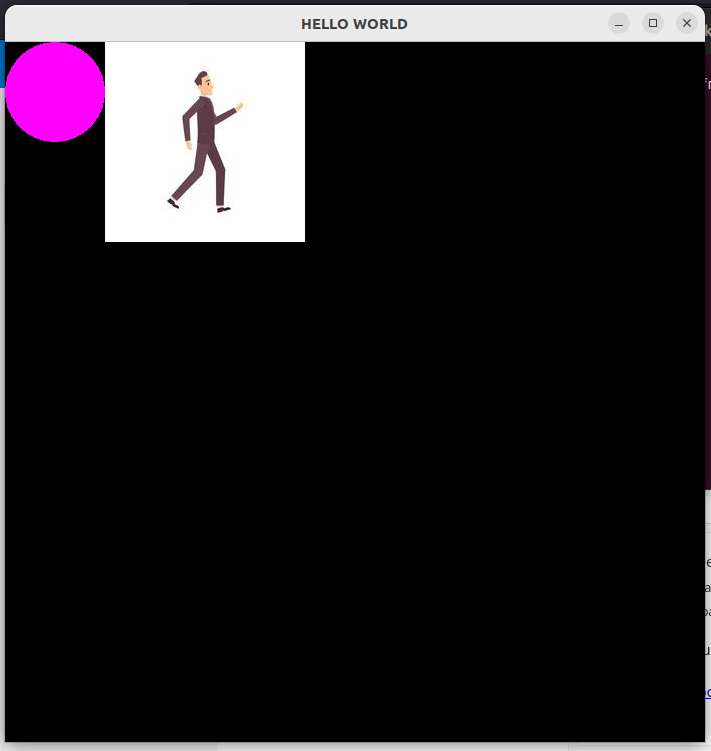
\includegraphics[width=0.5\textwidth]{ps0/Screenshot.png}
    \caption{Output of PS0 Assignment}
    \label{fig:ps0}
\end{figure}



\newpage
 
\newpage
\section{PS1a: Linear Feedback Shift Register}\label{sec:ps1a}
\graphicspath{{ps1a}}
\subsection{Discussion:}\label{sec:ps1a:disc}
       The ps1a assignment is an implementation of \textbf{LFSR(Linear Feedback shift Register) which is the Fibonacci LFSR}. This assignment is used for the ps1b i.e PhotoMagic. In this project, there are two main functions i.e, step() and generate(), The step() funtion is used for left shifting the one bit of the given seed, along the lsb is the result of the tap positions. These tap positions use the XOR operations and later it gives the lsb result.
    The generate() generates the states according to the given k inputs.\newline
    \textbf{XOR Truth Table:}
    \begin{center}
 \begin{tabular}{||c c c ||} 
 \hline
 A & B & Output \\ [0.5ex] 
 \hline\hline
 0 & 0 & 0 \\ 
 \hline
 0 & 1 & 1 \\
 \hline
 1 & 0 & 1 \\
 \hline
 1 & 1 & 0 \\ [1ex] 
 \hline
\end{tabular}
\end{center}


\subsection{Key algorithms, Data structures and OO Designs used in this Assignment:}\label{sec:ps1a:kdo}
        I have used string for the seed. Rather than using the xor operator I used the != operator as it works same and I have tried using it. I used simple string functions also. \newline
        \textbf{\colorbox{lime}{\textbf{The Tap position algorithm is as follows:}}}
 \begin{lstlisting}
 int _TAPbitvalue = funXOR(rgs[0], rgs[2]);
_TAPbitvalue = funXOR(_TAPbitvalue, funGetBit(rgs[3]));
_TAPbitvalue = funXOR(_TAPbitvalue, funGetBit(rgs[5]));
 \end{lstlisting}

\subsection{What I accomplished :}\label{sec:ps1a:accomplish}

I accomplished the full work of the LFSR and also both the important functions step() as well as generate() works completely fine. I learnt how to lint the program using the \textbf{cpplint.}

\subsection{What I already knew :}\label{sec:ps1a:knew}
 
I knew the concept of XOR and also I am well aware of how to shift the bits and also the concept of the MSB and LSB, as I have already taken Digital Logic design and Computer Architecture back in India.

\subsection{What I learned :}\label{sec:ps1a:learn}

I learned that how this LFSR is going to be used for the Image encoding and decoding of the Image in further part of the PS1 code. Where we utilize this part of assignment.

\subsection{Challenges :}\label{sec:ps1a:challenges}

To generate the LSB bit from the tap positions and re-attaching it to the seed was tough and also writing the new test case was challenging for me as I was new to the concept of the Boost Library.
\newpage

\subsection{Codebase}\label{sec:ps1a:code}

\colorbox{pink}{\textbf{Makefile:}} \newline \textbf{This Makefile is created by the referrence of the Version2 Makefile from the notes.}

\lstinputlisting[language=Make]{ps1a/Makefile}

\colorbox{pink}{\textbf{FibLFSR.cpp:}} \newline \textbf{This file contains the important methods such as step() and generate().}
\lstinputlisting{ps1a/FibLFSR.cpp}


\colorbox{pink}{\textbf{FibLFSR.h:}} \newline \textbf{this file is the header file for the above provided file "FibLFSR.cpp" . This file contains the initialization of the functions, libraries and variables.}

\lstinputlisting{ps1a/FibLFSR.h}

\colorbox{pink}{\textbf{test.cpp:}} \newline \textbf{This file is the test file which utilizes the <Boost Library> \newline
 The test cases are as follows: 
  \begin{itemize}
      \item At first case it was simple 16 bit seed (given)
    \item At second case it is random 20 bit seed
    \item At third case it is random 16 bit seed
  \end{itemize}}

\lstinputlisting{ps1a/test.cpp}


\newpage

\newpage
\section{PS1b: PhotoMagic}\label{sec:ps1b}
\graphicspath{{ps1b}}
\subsection{Discussion:}\label{sec:ps1b:disc}
The ps1b utilizes the ps1a i.e \textbf{LFSR: LINEAR FEEDBACK SHIFT REGISTER} as a supporting for the encoding and decoding of the image given as input.This project takes the input image i.e, Cat.png and Encrypts using the LFSR Randomizer and encrypts each and every pixel
of the image and saves to the cat-out.png file.
   For Encryption I used Common Example i.e; \newline
    \colorbox{yellow}{\textbf{./PhotoMagic cat.png cat-out.png 0011001100000 8}} \newline
    \textbf{Figure:\ref{fig:encode}} \newline
If we want to decrypt the encrypted image we write it as follows. \newline
    \colorbox{yellow}{\textbf{./PhotoMagic cat-out.png cat.png 0011001100000 8}} \newline
     \textbf{Figure: \ref{fig:decode}}
    
\subsection{Key algorithms, Data structures and OO Designs used in this Assignment:}\label{sec:ps1b:kdo}

I used The Vector STL in the LFSR as it is much easier to use and I felt flexible in it. Also Improvised the sample code to the Final code to get the perfect output. I used Image and its funtions and letter sent to Texture then to Sprite to draw on the window I used Two windows and two sprites for showing the difference between the normal cat image and the encoded and decoded image. The following code is used for the encoding and decoding: \newline
 \begin{lstlisting}
 void transform(sf::Image& kitty_image, FibLFSR* fibo){
	sf::Vector2u size = kitty_image.getSize();
	sf::Color color, newColor;

	for(int i = 0; i < size.x; i++){
		for(int j = 0; j < size.y; j++){
			color = kitty_image.getPixel(i, j);

			color.r = color.r xor fibo->generate(8);
			color.g = color.g xor fibo->generate(8);
			color.b = color.b xor fibo->generate(8);

			kitty_image.setPixel(i, j, color);	
		}
	}
}
 \end{lstlisting}

\subsection{Images used:}\label{sec:ps1b:img}
\begin{figure}[h]
    \centering
    
\includegraphics[width=0.45\textwidth]{ps1b/cat.png}
    \caption{Cat Image}
    \label{fig:mesh1}
\end{figure}


\subsection{What I accomplished :}\label{sec:ps1b:accomplish}

I accomplished the Encoding and Decoding of the Image using the C++ language in an efficient way. I have achieved using multiple windows, which was an amazing thing to do. 

\subsection{What I already knew :}\label{sec:ps1b:knew}

I knew how to take the input of the file and write to an output file. I already knew about how to create sprite using images and texture. I also knew how to display the windows and also to create the Makefile for the project.

\subsection{What I learned :}\label{sec:ps1b:learn}

I learned how to utilize two windows for the different output. I understood the concept of encoding and decoding using the pixels of the image and using the LFSR Randomizer. I also got to know about the mathematical calculations for the pixels.

\subsection{Challenges :}\label{sec:ps1b:challenges}

To find out the image pixels and the also to identify how to tranform them to the normal to encoded and then decode the image.

\subsection{Acknowledgements :}\label{sec:ps1b:ack}
\begin{itemize}
    \item \url{https://www.sfml-dev.org/tutorials/2.5/}
\end{itemize}
\newpage

\subsection{Codebase}\label{sec:ps1b:code}

\colorbox{pink}{\textbf{Makefile:}} \newline \textbf{This Makefile is contains no lint but it includes the flags as well as it is extension of the ps1a Makefile.}

\lstinputlisting[language=Make]{ps1b/Makefile}

\colorbox{pink}{\textbf{PhotoMagic.cpp:}} \newline \textbf{This file is the main file where the reading and writing also the encoding and decoding of the image takes place. This file gives the output in two windows. Input window and output window of the file.}
\lstinputlisting{ps1b/PhotoMagic.cpp}

\colorbox{pink}{\textbf{PhotoMagic.h:}}
\newline \textbf{This file contains the initializations and header files for the PhotoMagic.cpp}
\lstinputlisting{ps1b/PhotoMagic.h}
\newpage

\colorbox{pink}{\textbf{test.cpp:}}
\newline

\textbf{Given test file for the ps1a Assignment.}
\lstinputlisting{ps1b/test.cpp}

\newpage
\subsection{Output:}\label{sec:ps1b:output}
\begin{figure}[h]
    \centering
    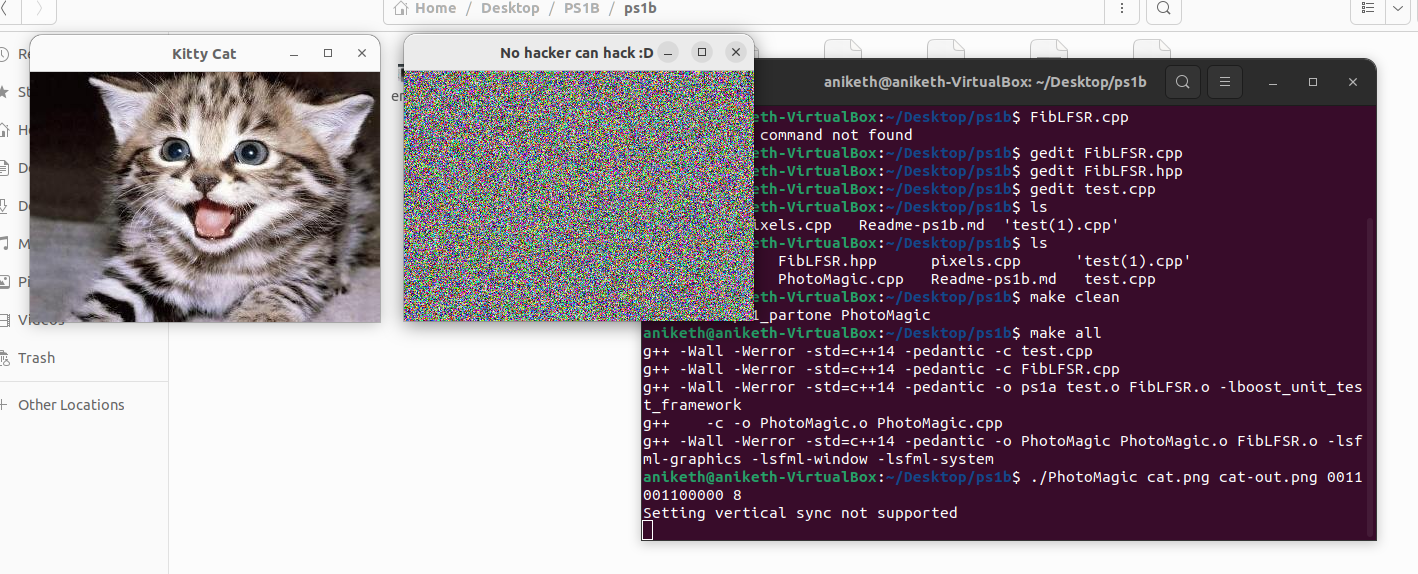
\includegraphics[width=1\textwidth]{ps1b/Encoded.png}
    \caption{Encoded Image}
    \label{fig:encode}
\end{figure}
\begin{figure}[h]
    \centering
    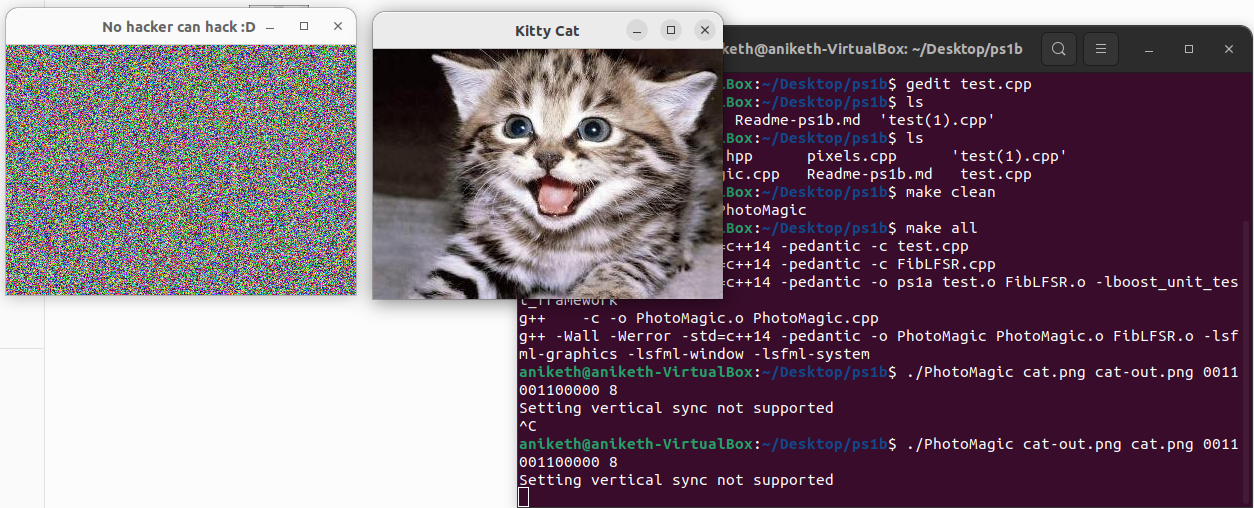
\includegraphics[width=1\textwidth]{ps1b/Decoded.png}
    \caption{Decode Image}
    \label{fig:decode}
\end{figure}


\newpage

\newpage
\section{PS2: Traingle Fractal}\label{sec:ps2}
\graphicspath{{ps2}}
\subsection{Discussion:}\label{sec:ps2:disc}
This Triangle Fractal is a variation of the Sierpinski triangle. The Polish mathematician Waclaw Sierpinski
described the pattern in 1915, but it has appeared in Italian art since the 13th century.

In this Assignment, We have to create a Triangle using only Recursion and display on the window by the help of the SFML.
We have to utilize the SFML Drawable class for the drawing of the Triangles. These traingles are similar to Sierpinski triangle but not the same. In this ps2, The triangles are created for the 3 sides of each and every triangle until unless the depth of the triangle becomes zero. The program should take two command line inputs, L and  N in that order:
\begin{itemize}
    \item L The length of the side of the base equilateral triangle (double)
    \item N The depth of the recursion (int)
\end{itemize}
\textbf{The command Line is as Follows: \newline
\colorbox{yellow}{./TFractal 200 5 } }

\subsection{Key algorithms, Data structures and OO Designs used in this Assignment:}\label{sec:ps2:kdo}
    I added Escape key to close the window as It was convenient.
    I made use of VertexArray to draw individual triangles themselves.
    The Triangle is completely draw until the depth value becomes zero.
    I added colors to the triangle.
    I Used cmath for the math functions.I added background to the triangle as you can see in the output \textbf{Figure: \ref{fig:tri}}
    \newline Changes I did: \newline
    \begin{itemize}
        \item   I made use of VertexArray for individual triangle.
\item  Implemented different Mathematic formulas.
\item  Added Background to the Triangle.
\item  Added Cpplint to target file.
\item  Used randr() rather than rand()
    \end{itemize}
    \textbf{\colorbox{lime}{Recursive method used in ftree:}} 
    \begin{lstlisting}
fTree(tris, len / 2, depth - 1, _xcen_a, ycenter_a);
fTree(tris, len / 2, depth - 1, _xcen_b, ycenter_b);
fTree(tris, len / 2, depth - 1, _xcen_c, ycenter_c);
    \end{lstlisting}
    \textbf{\colorbox{lime}{Random Color Code:}}
    \begin{lstlisting}
    int v1 = rand_r(&range) % 255;
int v2 = rand_r(&range) % 255;
int v3 = rand_r(&range) % 255;
triangle[0].position = sf::Vector2f(xvertex_a , yvertex_a);
triangle[0].color = sf::Color(v1 , v2 , v3);
triangle[1].position = sf::Vector2f(xvertex_b , yvertex_b);
triangle[1].color = sf::Color(v1 , v2 , v3);
triangle[2].position = sf::Vector2f(xvertex_c , yvertex_c);
triangle[2].color = sf::Color(v1 , v2 , v3);
triangle[3].position = triangle[0].position;
triangle[3].color = sf::Color(v1 , v2 , v3);
    \end{lstlisting}
    \newpage

\subsection{Images used:}\label{sec:ps2:img}
\begin{figure}[h]
    \centering
    
\includegraphics[width=0.5\textwidth]{ps2/backg.jpg}
    \caption{Background for the Triangle}
    \label{fig:decode}
\end{figure}


\subsection{What I accomplished :}\label{sec:ps2:accomplish}

I have accomplished the creation of the Triangle Fractal using the Recursive methods. It was really an Amazing and effective way to create patterns using recursion. I have added random colors for it to gain extra credit.

\subsection{What I already knew :}\label{sec:ps2:knew}

I already knew how to create a window and few events. I also knew how to add background to the window and set the window size. I also knew how to take command line arguments.

\subsection{What I learned :}\label{sec:ps2:learn}

I learned how to implement the sf::Drawable class in much efficient manner. I also got to know how to utilize the mathematic functions and recursive methods to draw amazing patterns.

\subsection{Challenges :}\label{sec:ps2:challenges}

To find out the exact math formula and align the triangle to the center was the challenging part.
\newpage
\subsection{Codebase}\label{sec:ps2:code}

\colorbox{pink}{\textbf{Makefile:}} \newline \textbf{This Makefile contains the linting too.}
\lstinputlisting[language=Make]{ps2/Makefile}

\colorbox{pink}{\textbf{TFractal.cpp}} \newline \textbf{This file is important as the Recursion takes place as well as the window is drawn. It calls the Triangle.cpp for creating the Triangles until unless the depth becomes zero.}
\lstinputlisting{ps2/TFractal.cpp}

\colorbox{pink}{\textbf{Triangle.h}} \newline \textbf{It is a header file where the initialization of libraries as well as variables and methods takes place.}
\lstinputlisting{ps2/Triangle.h}

\newpage

\colorbox{pink}{\textbf{Triangle.cpp}} \newline \textbf{This file utilizes the SFML library to create the Triangles.}
\lstinputlisting{ps2/Triangle.cpp}





\subsection{Output:}\label{sec:ps2:output}
\begin{figure}[h]
    \centering
    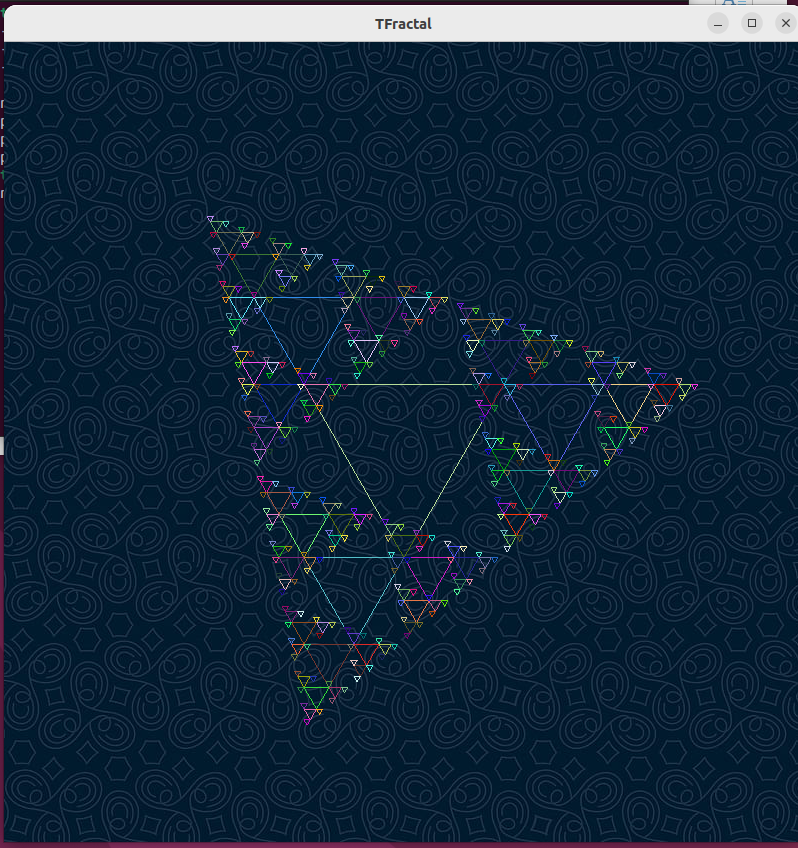
\includegraphics[width=0.7\textwidth]{ps2/screenshot.png}
    \caption{Triangle TFractal}
    \label{fig:tri}
\end{figure}

\newpage

\newpage
\section{PS3a: N-Body Simulation (Static)}\label{sec:ps3a}
\graphicspath{{ps3a}}
\subsection{Discussion:}\label{sec:ps3a:disc}
We have been through our school education where we learned about solar systems. We wondered how these planets are implemented as an animation to display on the screen. Well to answer these thoughts, such assignments are created to know how to create animation. At the first part we will create a static animation of the solar system and in the second part we will simulate the static bodies by using physics.


    The \textbf{PS3a} asks us to load and display static images of the planets.
    We are using two classes Universe and CelestialBody classes. The class CelestialBody is used to show any planet rendered in the universe, example: Our planet Earth. Universe class has a vector of CelestialBody and has a function to create the entire universe by accessing the vector.
    
    \textbf{We use the provided planets.txt file for this assignment: The values are as follows: } \newline
    \textbf{Inputs: 5 \newline Radius: 2.50e+11 }
    \begin{center}
 \begin{tabular}{||c c c c c c||} 
 \hline
 x-axis & y-axis & velocity of x-axis & velocity of y-axis & Mass & filename \\ [0.5ex] 
 \hline\hline
 1.4960e+1 & 0.0000e+00 & 0.0000e+00 & 2.9800e+04 & 5.9740e+24 &  earth.gif  \\ 
 \hline
 2.2790e+11 & 0.0000e+00 & 0.0000e+00 & 2.4100e+04 & 6.4190e+2 &  mars.gif  \\ 
 \hline
 5.7900e+10 & 0.0000e+00 & 0.0000e+00 &  4.7900e+04 &  3.3020e+23 &  mercury.gif  \\ 
 \hline
0.0000e+00 & 0.0000e+00 & 0.0000e+00 & 0.0000e+00 & 1.9890e+30 &  sun.gif  \\ 
 \hline
1.0820e+11  & 0.0000e+00 & 0.0000e+00 & 3.5000e+04 & 4.8690e+24 &  venus.gif  \\  
 \hline
\end{tabular}
\end{center}



\subsection{Key algorithms, Data structures and OO Designs used in this Assignment:}\label{sec:ps3a:kdo}
I used istream to read the data from planets.txt and ostream as output.Displays the planets in an SFML window.
       Reads input of file using < operator.  
       I did not use any smart pointers. Just used General Pointers.
       Simply added (space) key to exit from the window.
       used Address-operator for managing the addresses of variables and also the objects.
       I have not used any smart pointers. \newline
       \textbf{\colorbox{lime}{istream code:}}
       \begin{lstlisting}
       std::istream& operator>> (std::istream &data, CelestialBody &body) {

data >> body.x >> body.y >> body.vx >> body.vy >> body.mass >> body.filename;

if (!body.image.loadFromFile(body.filename))
    return data;
body.calculatePosition();
body.texture.loadFromImage(body.image);
body.sprite.setTexture(body.texture);
body.sprite.setPosition(body.rx, body.ry);
return data;

}
       \end{lstlisting}
              \textbf{\colorbox{lime}{ostream code:}}
       \begin{lstlisting}
       std::ostream& operator<< (std::ostream &outstream, CelestialBody &body){
outstream << "CelestialBody :  x:" << body.x << " y:";
outstream << body.y << " velx:" << body.vx << " vely:";
outstream << body.vy << " mass:" << body.mass << "";
outstream << " ~~x:" << body.rx << "  --- " << body.ry << "~~" << " " << body.filename << std::endl;
return outstream;
       \end{lstlisting}

\subsection{Images used:}\label{sec:ps3a:img}
\begin{figure}[h]
    \centering
    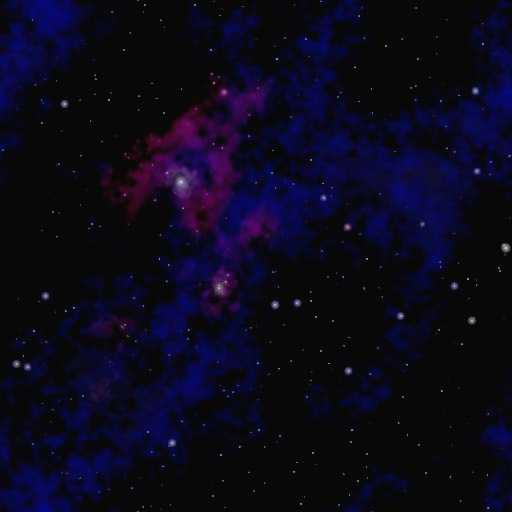
\includegraphics[width=0.5\textwidth]{ps3a/starfield.jpg}
    \caption{Background Image}
    \label{fig:ps3abg}
\end{figure}
\begin{figure}[h]
    \centering
    
\includegraphics[width=0.2\textwidth]{ps3a/earth.png}
    \caption{Background Image}
    \label{fig:earth}
\end{figure}
\begin{figure}[h]
    \centering
    
\includegraphics[width=0.2\textwidth]{ps3a/mars.png}
    \caption{Background Image}
    \label{fig:mars}
\end{figure}
\newpage
\begin{figure}[h]
    \centering
    
\includegraphics[width=0.2\textwidth]{ps3a/venus.png}
    \caption{Background Image}
    \label{fig:venus}
\end{figure}\begin{figure}[h]
    \centering
    
\includegraphics[width=0.2\textwidth]{ps3a/sun.png}
    \caption{Background Image}
    \label{fig:sun}
\end{figure}
\begin{figure}[h]
    \centering
    
\includegraphics[width=0.2\textwidth]{ps3a/mercury.png}
    \caption{Background Image}
    \label{fig:mercury}
\end{figure}
\newpage
\subsection{What I accomplished :}\label{sec:ps3a:accomplish}

I accomplished creating a solar system by the given input data. I created my first animated solar system. I am amazed that how physics can be implemented in the code.

\subsection{What I already knew :}\label{sec:ps3a:knew}

I knew how to add the background and use of the draw. I also knew how to take input from the file and display.
I knew how to create header files and implement them into the cpp files.


\subsection{What I learned :}\label{sec:ps3a:learn}

I learnt how to use physics in creating the solar model. I understood much use of the istream and ostream in this assignment. I understood the calculations required for the placement of the CelestialBodies.
         I was able to learn how to use unitary methods and also vectors in a good level.
         Honestly, I was weak in operator overloading but by doing this project I am able to grip on it.

\subsection{Challenges :}\label{sec:ps3a:challenges}
        I was unable to use smart pointers and few algorithm classes, so I kind of felt a difficulty in that.

\subsection{Acknowledgments :}\label{sec:ps3a:ack}
\textbf{Links :}
\begin{itemize}
    \item \url{https://www.sfml-dev.org/tutorials/2.5/graphics-sprite.php}
    \item \url{https://icarus.cs.weber.edu/~dab/cs1410/textbook/11.Operators/io_overload.html}
    \item \url{https://www.cplusplus.com/reference/vector/vector/}
    \item \url{https://www.sfml-dev.org/documentation/2.5.1/classsf_1_1Drawable.php}
    \item \url{https://stackoverflow.com/questions/34458791/making-custom-types-drawable-with-sfml}
\end{itemize}
\newpage


\subsection{Codebase}\label{sec:ps3a:code}

\textbf{\colorbox{pink}{Makefile}} \newline \textbf{This Makefile has no Linting as the program does not have any lints.}
\lstinputlisting[language=Make]{ps3a/Makefile}

\textbf{\colorbox{pink}{main.cpp}} \newline \textbf{The main file is important as it is base for creating a window and displaying the CelestialBodies on it.}
\lstinputlisting{ps3a/main.cpp}

\textbf{\colorbox{pink}{CelestialBody.hpp}} \newline \textbf{The CelestialBody.hpp contains the initializations of istream,ostream and variable and methods for the creation of the Nbodies.}
\lstinputlisting{ps3a/CelestialBody.hpp}

\newpage
\textbf{\colorbox{pink}{CelestialBody.cpp}} \newline \textbf{This is the file where the Celestial body data are taken by the istream and provide an accurate calculation for the position of them as well as provide the data of each CelestialBody on the terminal.}
\lstinputlisting{ps3a/CelestialBody.cpp}

\textbf{\colorbox{pink}{Universe.hpp}} \newline \textbf{This header file contains the declarations of few important variables such as numberOFplanets,radius and also methods.}
\lstinputlisting{ps3a/Universe.hpp}


\textbf{\colorbox{pink}{Universe.cpp}} \newline \textbf{This file sets radius and adds Body to window}
\lstinputlisting{ps3a/Universe.cpp}


\newpage
\subsection{Output:}\label{sec:ps3a:output}
\begin{figure}[h]
    \centering
    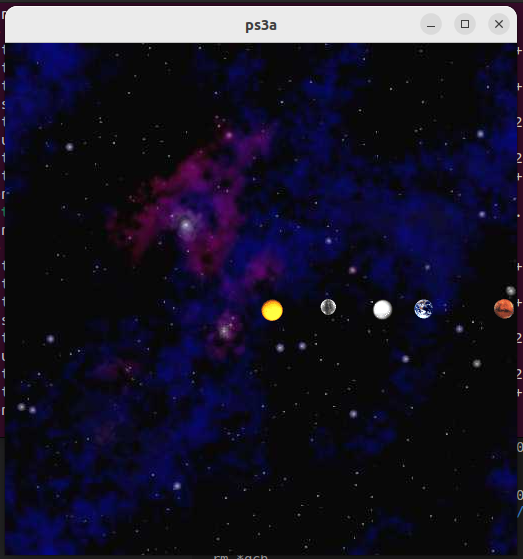
\includegraphics[width=1\textwidth]{ps3a/screenshot.png}
    \caption{NBody Simulation (static)}
    \label{fig:ps3a}
\end{figure}

\newpage

\newpage
\section{PS3b: N-Body Simulation}\label{sec:ps3b}
\graphicspath{{ps3b}}
\subsection{Discussion:}\label{sec:ps3b:disc}
    In this project we are simulating the created solar system in \textbf{ps3a} by using physics in it. Basic physics such as net force, Acceleration , Pair-wise forces and their formulas.
    According to the given simulating time and time step the Planets Revolve around the sun.
    \newline By default the detail code. \newline
    \textbf{\colorbox{yellow}{ ./NBody 157788000.0 25000.0 < planets.txt }}

\subsection{Key algorithms, Data structures and OO Designs used in this Assignment:}
      The smart pointers that I have implemented in this project and improved the previous ps3a code.
     I have studied the notes of class as well as few physics site to actaully get the correct physics formula to run.
 I used smart pointers to mange the memory locations of variables as well as objects in CelestialBody and Universe classes. I also used the classic vector for the memory management in the project. There was much utilizations of the Physic laws for creating a simulation of this project.

\subsection{Images used:}
The images are already shown in PS3a Sections, To browse them you can click on the following \textit{Figure Numbers:}
\begin{itemize}
    \item \textbf{The Background is Figure \ref{fig:ps3abg}}
    \item \textbf{The Earth is Figure \ref{fig:earth}}
    \item \textbf{The Mars is Figure \ref{fig:mars}}
    \item \textbf{The Venus is Figure \ref{fig:venus}}
    \item \textbf{The Sun is Figure \ref{fig:sun}}
    \item \textbf{The Mercury is Figure \ref{fig:mercury}}
    
\end{itemize}

\subsection{What I accomplished :}

I accomplished creating a full animated solar system using C++ SFML library. I have also used audio for the window for (extra point).

\subsection{What I already knew :}

I already knew how to read data from the given input file. I was well aware of the SFML library to draw bodies and put the background to it.

\subsection{What I learned :}

I learnt how physics can be the part of the computer field. It enlightened me in using different the formulas of physics in different aspects of the functions in this assignment. By doing this assignment's extra credit, I got to know how to create different solar system as well how to implement audio into the window of the SFMl.

\subsection{Challenges :}
       At starting of the simulation i have a glitch in my sound, I Guess that the convertion of mp3 to wav was not good enough, or may be other reason.
       Linting became challenging for me in this assingment.

\subsection{Codebase}\label{sec:ps3b:code}

\textbf{\colorbox{pink}{Makefile}} \newline \textbf{This Makefile has no Linting as the program does not have any lints.}
\lstinputlisting[language=Make]{ps3b/Makefile}

\textbf{\colorbox{pink}{main.cpp}} \newline \textbf{The main file is important as it is base for creating a window and displaying the CelestialBodies on it.In addition, in this part-b I have added more functions to make a simulation of these CelestialBodies. Moreover, I added audio and Time Elapsed to the SFML window.}
\lstinputlisting{ps3b/main.cpp}

\textbf{\colorbox{pink}{CelestialBody.hpp}} \newline \textbf{The CelestialBody.hpp contains the initializations of istream,ostream and variable and methods for the creation of the Nbodies. In this part-b, I have also added File eXceptions and more functions as to achieve the simulation of the planets.}
\lstinputlisting{ps3b/CelestialBody.hpp}

\textbf{\colorbox{pink}{CelestialBody.cpp}} \newline \textbf{This is the file where the Celestial body data are taken by the istream and provide an accurate calculation for the position of them as well as provide the data of each CelestialBody on the terminal.}
\lstinputlisting{ps3b/CelestialBody.cpp}

\textbf{\colorbox{pink}{Universe.hpp}} \newline \textbf{This header file contains the declarations of few important variables such as numberOFplanets,radius and also methods. In part-b, we added istream and ostream to it.}
\lstinputlisting{ps3b/Universe.hpp}


\textbf{\colorbox{pink}{Universe.cpp}} \newline \textbf{The universe file in part-b has also played a major role in case of calculating scaleForce, Netforce and organizing the Bodies while they are revolving along the orbit provided.}
\lstinputlisting{ps3b/Universe.cpp}


\subsection{Output:}
\textbf{To see the static Output got to Figure: \ref{fig:ps3a}}

\subsection{Acknowledgements:}
\begin{itemize}
    \item  \url{ https://docs.microsoft.com/en-us/cpp/cpp/smart-pointers-modern-cpp?view=msvc-170}
  \item \url{https://www.geeksforgeeks.org/vector-in-cpp-stl/}
  \item \url{https://study.com/learn/lesson/net-force-formula-examples-how-find.html}
  \item \url{https://www.sfml-dev.org/tutorials/2.5/audio-sounds.php}
\end{itemize}
\newpage

\newpage
\section{PS4a: CircularBuffer}\label{sec:ps4a}
\graphicspath{{ps4a}}
\subsection{Discussion:}\label{sec:ps4a:disc}
 The ps4a assignment creates a circular buffer which will be used for the follow up assignment ps4b. In this assignment, we create basically a circular queue, where the head and tail will be connected and follows the same mechanism as queue i.e, FIFO (First In First Out) Mechanism. 
 \begin{figure}[h]
    \centering
    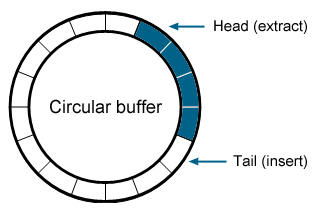
\includegraphics[width=1\textwidth]{ps4a/cb.jpg}
    \caption{Circular Buffer}
    \label{fig:cb}
\end{figure}
\subsection{Key algorithms, Data structures and OO Designs used in this Assignment:}
 I make use of Vectors in standard manner rather than the functions as I found it amusing and easy to understand theoratically, Where I used basic rules such as initial head, tail.
 I used the default format of the pdf to create the template version and also added few functions such as print etc.
 I used exceptions to inform the provided arised exceptions.

\subsection{What I accomplished :}

I have created a CircularBuffer using the vector. It works properly and gives the output too in the main function. I have used the templates so therefore there is no need for .cpp file. 

\subsection{What I already knew :}

I knew how to implement template. I was aware of the CircularBuffer concept as I did a Circular buffer program without using templates in my Data Structure Class.

\subsection{What I learned :}

I learnt how to implement vector and the template in an efficient way.

\subsection{Challenges :}

To implement template throughout the code as well as implementing in the test file was quite a challenge for me.

\subsection{Codebase}\label{sec:ps4a:code}

\textbf{\colorbox{pink}{Makefile:}} \newline \textbf{This Makefile has linting included.}

\lstinputlisting[language=Make]{ps4a/Makefile}

\textbf{\colorbox{pink}{CircularBuffer.h:}} \newline \textbf{This file is the important file as it contains all the methods for the CircularBuffer to run. It does not have a cpp file as I have utilized the template.}
\lstinputlisting{ps4a/CircularBuffer.h}

\textbf{\colorbox{pink}{main.cpp:}} \newline \textbf{This file is just for the output of the sample input and methods of the CircularBuffer}
\lstinputlisting{ps4a/main.cpp}

\newpage
\textbf{\colorbox{pink}{test.cpp: }} \newline \textbf{The test file tests for the Exceptions as well as all the functions of the CircularBuffer as you can see in the output section.}
\lstinputlisting{ps4a/test.cpp}

\subsection{Output :}
\begin{figure}[h]
   \centering
    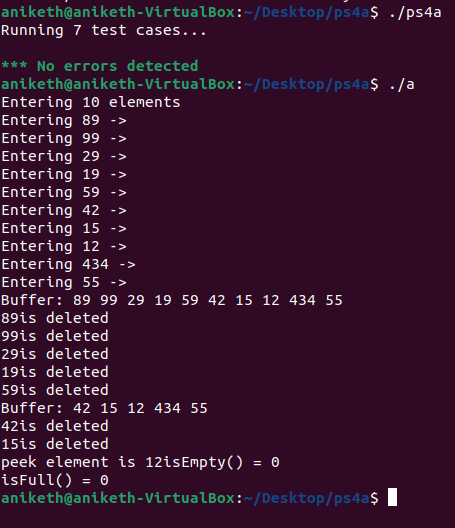
\includegraphics[width=1\textwidth]{ps4a/ps4a.png}
    \caption{PS4a Output in Terminal}
    \label{fig:ps4a}
\end{figure}


\newpage

\newpage
\section{PS4b: StringSound}\label{sec:ps4b}
\graphicspath{{ps4b}}
\subsection{Discussion:}\label{sec:ps4b:disc}
   This Project produces sound using the SFML library <Audio>, Where we produces notes by using our keys. We utilize the ps4a CircularBuffer in this project.
   Basic motto of this project is to create a simulation of guitar plucking, but as I wanted to do extra credit, I made a Piano simulation note, It is not accurate but close.
   Main thing in this project is using the Karplus-Strong algorithm.

\subsection{Key algorithms, Data structures and OO Designs used in this Assignment:}

The Vector is used for the samples and also creating a sound buffer and holding the sounds bpm. Basic switch method is used for taking the inputs of keys and sending them to calculate the frequency and return with a audio. There are much use of new functions in creating this assignment.

\subsection{Images used:}
\begin{figure}[h]
   \centering
    
\includegraphics[width=0.4\textwidth]{ps4b/backg.jpg}
    \caption{Jazz Background}
    \label{fig:bgps4b}
\end{figure}


\subsection{What I accomplished :}

I accomplished producing piano sounds by altering the frequency. It is an amazing project to create our own instrument using C++.

\subsection{What I already knew :}

I knew how to implement few math functions as well as basics of the SFML.

\subsection{What I learned :}
I learnt how the frequency can be use to create different instruments. I understood how to take the sample inputs from keyboard and produce sound.
\subsection{Challenges :}
Finding out the right frequency and implementing of the samples by reading from the keys was difficult challenge to me.

\subsection{Codebase}\label{sec:ps4b:code}

\textbf{\colorbox{pink}{Makefile}} \newline \textbf{This Makefile contains the lint and is extension of the PS4a Makefile.}

\lstinputlisting[language=Make]{ps4b/Makefile}

\textbf{\colorbox{pink}{KSGuitarSim.cpp}} \newline \textbf{This is the main file where the Samples are taken and window is drawn as well as where takes inputs from keyboard and produces sound.}
\lstinputlisting{ps4b/KSGuitarSim.cpp}

\newpage
\textbf{\colorbox{pink}{StringSound.h}} \newline \textbf{The initialization of the StringSound methods and variables.}
\lstinputlisting{ps4b/StringSound.h}

\textbf{\colorbox{pink}{StringSound.cpp}} \newline \textbf{The frequency is blent in and produces the sound required according to the frequency.}
\lstinputlisting{ps4b/StringSound.cpp}


\subsection{Output:}
\begin{figure}[h]
   \centering
    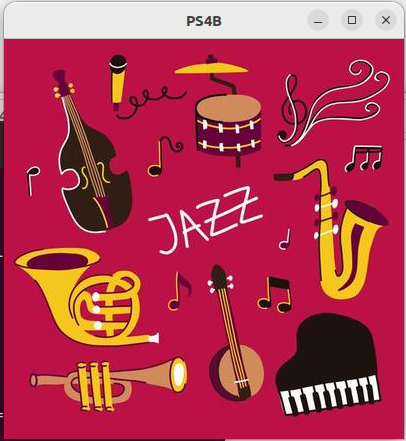
\includegraphics[width=0.69\textwidth]{ps4b/ps4b.png}
    \caption{PS4b Output Window}
    \label{fig:ps4b}
\end{figure}


\newpage

\newpage
\section{PS6: Random Writer}\label{sec:ps6}
\graphicspath{{ps6}}
\subsection{Discussion:}\label{sec:ps6:disc}
 The Markov Model predicts the next characters in a sequence of k length words called kgrams.
 The RandWriter class takes a string and order k as input and maps each kgram in the string to each
 character following that kgram and it's frequency.
 This class can now generate strings of any given length, using the kgrams that have been seen before.
 The string's characters are based on the probabilities of the k-length strings that were stored in the hashmap.
 \newline
 \textbf{I used the given structure in this assignment:}
 \begin{lstlisting}
 class RandWriter {
public:

RandWriter(string text, int k);
int orderK() const; // Order k of Markov model
// Number of occurences of kgram in text
// Throw an exception if kgram is not length k
int freq(string kgram) const;
// Number of times that character c follows kgram
// if order=0, return num of times that char c appears
// (throw an exception if kgram is not of length k)
int freq(string kgram, char c) const;
// Random character following given kgram
// (throw an exception if kgram is not of length k)
// (throw an exception if no such kgram)
char kRand(string kgram);

string generate(string kgram, int L);
}

 \end{lstlisting}

\subsection{Key algorithms, Data structures and OO Designs used in this Assignment:}
RandWriter's constructor takes a string and and the order of the kgrams as input.
It initializes and constructs the hashmap.
The kRand function generates a string of length n, using the hashmap that was generated.
The function just iterates through a kgram's character map (the nested, inner map) and appends them in a string.
Then it randomly returns a char from this string.
The freq function returns the frequency of a kgram by searching/traversing the string.
The second overloaded function returns the frequency of a character, which is simple and just looks it up in the hashmap;
> return ktable.at(kgram).at(c);
The generate function generates a new string by just calling the rand function, until the desired output length is reached.


\subsection{What I accomplished :}

I have accomplished to implement Markov Model. I have created a working Random Writer.

\subsection{What I learned :}

I have learnt about the Markov model and how it works. Also learnt about the Hash Map.

\subsection{Challenges :}

Implementing the Markov Model was Challenging for me.

\subsection{Codebase}\label{sec:ps6:code}

\textbf{\colorbox{pink}{Makefile :}} \newline \textbf{This Makefile contains the lint.}
\lstinputlisting[language=Make]{ps6/Makefile}

\textbf{\colorbox{pink}{TextWriter.cpp :}} \newline \textbf{This file is important as it takes command line arguments and also gives you the output.}
\lstinputlisting{ps6/TextWriter.cpp}

\textbf{\colorbox{pink}{RandWriter.h :}} \newline \textbf{The initialization of variables and methods.}
\lstinputlisting{ps6/RandWriter.h}
\newpage

\textbf{\colorbox{pink}{RandWriter.cpp :}} \newline \textbf{The important functions for the Markov Model are implemented in this file.}
\lstinputlisting{ps6/RandWriter.cpp}




\textbf{\colorbox{pink}{test.cpp :}} \newline \textbf{The test file tests for the given input as well as runtimeerror exception}
\lstinputlisting{ps6/test.cpp}


\newpage

\newpage
\section{PS7: Kronos Log Parsing}\label{sec:ps7}
\graphicspath{{ps7}}
\subsection{Discussion:}\label{sec:ps7:disc}
    We analyze the Kronos Intouch time clock log by using regular expressions to parse the file.
    Also we verify device boot up timing.
    here we take the given device[1-6]*underscore*intouch.log files and give a resultant file which contains the time, date, status and line number of the boot to the .rpt file.

\subsection{Key algorithms, Data structures and OO Designs used in this Assignment:}
    I used the lambda expression for getting the time from first 19 characters i.e substring(0,19).
    I prefer using lambda expression than ordinary method as its more efficient.
    Just utilized the three functions from the regex library to finish my project.
\subsection{Explanation of the code:}
    Firstly, I initialize regular expressions to the starting and ending log entries so it can be used to compare the regex to find.
    if there is a match in every line of the file(.log). I create an -outputfile where the data of the result is stored as filename.log.rpt .There is a use of bool exp to keep tracking of the incomplete booting. I utilize the regex-search function to search a match for the starting regular expression(log.c.166). 
    if there is no incomplete booting, I write the date,time,line number and status of the boot to our -outputfile. The else if condn is used to search the line for finding the match for the ending regular expression. if that is found, The calculation of the duration of the time is begun by using posix. Again I write the line-number, date , time and duration it took for the completion of sequence.

\subsection{What I accomplished :}

I accomplished creating Kronos log Parsing and approach towards regular expression in C++.

\subsection{What I learned :}

I learnt implementing of the regex library <regex> More efficiently.\newline
I have implemented following regex functions into my code. \newline
\begin{itemize}
    \item boost::regex startMessage("( \\(log.c.166\\) server started)");
    \item boost::regex endMessage("(oejs.AbstractConnector:Started SelectChannelConnector)");
    \item regex-search(s, startMessage)
   \item  regex-search(s, endMessage)
\end{itemize}

\subsection{Challenges :}

Implementing a proper format was challenging to me to the output file.

\subsection{Codebase}\label{sec:ps7:code}

\textbf{\colorbox{pink}{Makefile:}} \newline \textbf{This Makefile has lint.}
\lstinputlisting[language=Make]{ps7/Makefile}

\textbf{\colorbox{pink}{main.cpp:}} \newline \textbf{The main file contains all the regex library as well as time library and functions to achieve the \textit{Kronos Log Parsing}}
\lstinputlisting{ps7/main.cpp}


\subsection{Output:}
\begin{figure}[h]
   \centering
    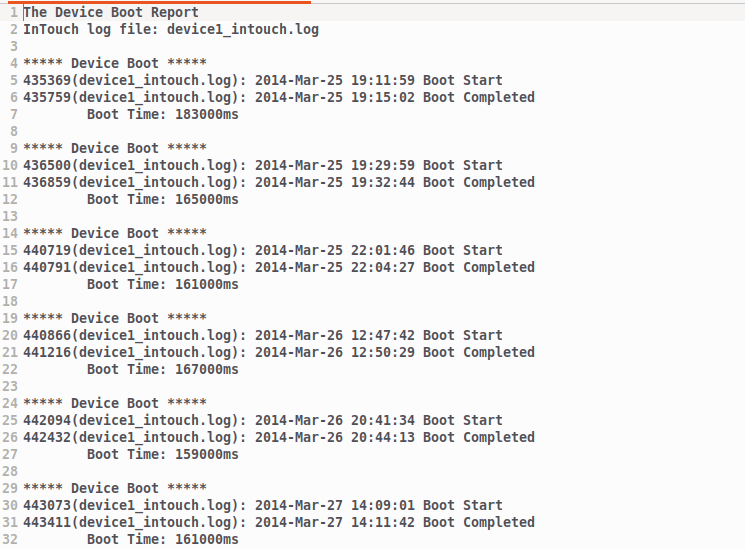
\includegraphics[width=1\textwidth]{ps7/d1.png}
    \caption{device1 output}
    \label{fig:ps7d1}
\end{figure}
\begin{figure}[h]
   \centering
    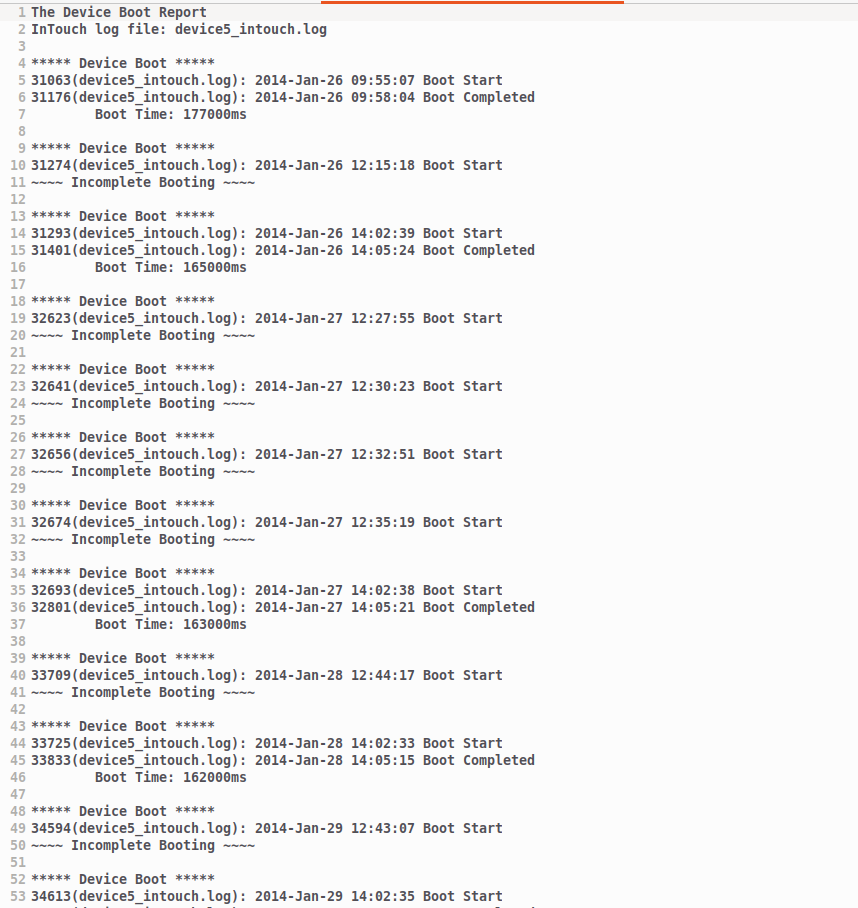
\includegraphics[width=1\textwidth]{ps7/d5.png}
    \caption{device5 output}
    \label{fig:ps7d5}
\end{figure}
\begin{figure}[h]
   \centering
    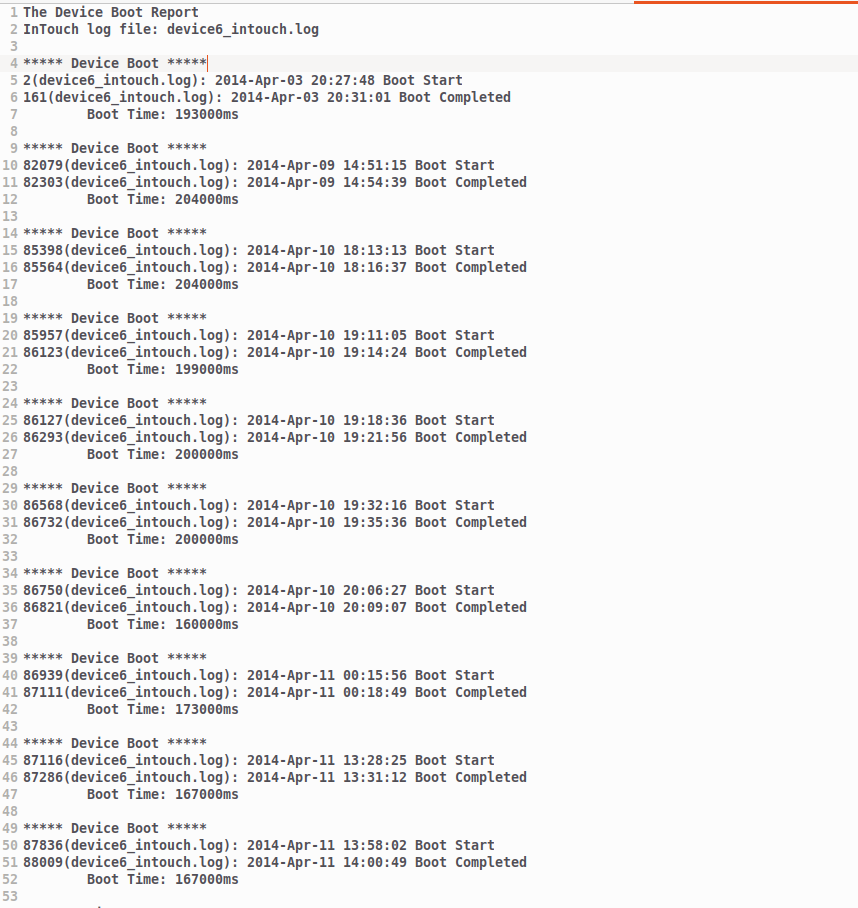
\includegraphics[width=1\textwidth]{ps7/d6.png}
    \caption{device6 output}
    \label{fig:ps7d6}
\end{figure}

\newpage



\end{document}
